\documentclass[11pt]{article}

%Both greek and english language support
\usepackage[greek,english]{babel}
\usepackage[utf8]{inputenc}
\usepackage{alphabeta}

% For \includegraphics
\usepackage{graphicx}   
\usepackage[space]{grffile}

\usepackage{amsmath}
\usepackage{amssymb}
\usepackage{float}

\usepackage[makeroom]{cancel}
\usepackage[colorinlistoftodos]{todonotes}

% For hyper links
\usepackage[unicode]{hyperref}

%Diagonal line on Tables\documentclass[11pt]{article}
\usepackage{diagbox}

%Multiple rows in tables
\usepackage{multirow}

% %----------------------------- MATLAB -----------------------------
\usepackage[T1]{fontenc}
% \usepackage{bigfoot} % to allow verbatim in footnote
\usepackage[numbered,framed]{matlab-prettifier}

\lstset{
  style              = Matlab-editor,
  basicstyle         = \mlttfamily,
  escapechar         = ",
  mlshowsectionrules = true,
}
\let\ph\mlplaceholder % shorter macro
\lstMakeShortInline"

% % In order to use Matlab code just use this 
% \begin{lstlisting}[caption = {Title}]
%   code
% \end{lstlisting}
% %----------------------------- MATLAB -----------------------------

% Page margins 
\usepackage{geometry}
 \geometry{
 a4paper,
 total={170mm,257mm},
 left=20mm,
 top=20mm,
 }

\DeclareUnicodeCharacter{2212}{-}   %Negative exponential


\begin{document}
    %--------------------------------------------------------------------------------------------
    % Title Page
    \begin{titlepage}
        \center
        %----------------------------------------------------------------------------------------
        %	HEADING SECTIONS
        \textsc{\LARGE Technical University of Crete}\\[2cm] 
        \Large Τηλεπικοινωνιακά Συστήματα Ι\\[1cm] 
        
        \rule{\linewidth}{0.5mm} \\[0.5cm]
            { \huge \bfseries Άσκηση 2}\\[0.5cm]
        \rule{\linewidth}{0.5mm} \\[2.5cm]
        
        \begin{minipage}{0.4\textwidth}
            \begin{flushleft} \large
                \emph{Author:}\\
                    Σπυριδάκης Χρήστος
            \end{flushleft}
        \end{minipage}
        ~
        \begin{minipage}{0.4\textwidth}
            \begin{flushright} \large
                \emph{ΑΜ:} 2014030022
            \end{flushright}
        \end{minipage}\\[4cm]
        
        {\large November 28, 2019}\\[2cm] 
        %----------------------------------------------------------------------------------------
        %	LOGO
        
\includegraphics[scale=0.5]{TUC.png} 
        \vfill
    \end{titlepage}



    % %-------------------------------------
    % %   A. subsection
    % \subsection*{A. }
    % Εισαγωγή: 
    
    % \begin{figure}[H]
    %     \centering
    %     \includegraphics[scale=0.5, width=0.8\textwidth]{photos/} \\
    %     \caption{}
    % \end{figure}
    
    % \begin{lstlisting}[caption = {}]
    %     code
    % \end{lstlisting}
    % \par \noindent
    % Συμπεράσματα:
    
    

    % \par \noindent
    %-------------------------------------------------------------------------
    %   Eisagwgi
    \section*{Εισαγωγή}
    Για την διευκόλυνση της υλοποίησης είναι καλό να σημειωθεί ότι το κάθε μέρος υλοποιήθηκε σε διαφορετικό script, αυτό είχε τα θετικά του, στο να είναι περισσότερο διακριτός ο κώδικας για ανάπτυξη και αποσφαλμάτωση, αλλά χρειάστηκε να ξανά δημιουργηθούν σήματα που είχαν δημιουργηθεί σε προηγούμενα ερωτήματα. Δεν επηρεάζονται κάπως τα αποτελέσματα απλά είναι μία διευκρίνηση σχετικά με την δομή που δόθηκε στον κώδικα. 
    \par \noindent
    Επίσης παρατηρήθηκε ότι κατά την διάρκεια της άσκησης είναι πολλά πράγματα τα οποία μοιάζουν μεταξύ των ζητουμένων. Ακολουθήθηκε λοιπόν μία τακτική δομημένου προγραμματισμού με χρήση συναρτήσεων, προκειμένου ενέργειες που ζητούνται από περισσότερο του ενός σημεία, να μην επαναλαμβάνονται από το μηδέν. Για αυτό το λόγο υπάρχουν πολλαπλά βοηθητικά αρχεία τα οποία δημιουργήθηκαν. Σε κάθε ενότητα όπως χρειάζεται θα εισαγάγεται η λειτουργικότητα της κάθε συνάρτησης που περιέχεται σε ένα αρχείο και στην συνέχεια θα δείχνεται μόνο ο τρόπος κλήσης της. Τα αρχεία τα οποία υπάρχουν συνολικά για την ολοκληρωμένη εκτέλεση της άσκησης είναι τα εξής: \emph{\texttt{srrc\_pulses.m}}, \emph{\texttt{part\_a.m}}, \emph{\texttt{part\_b.m}}, \emph{\texttt{bits\_to\_2PAM.m}}, \emph{\texttt{bits\_to\_4PAM.m}}, \emph{\texttt{create\_xt.m}}, \emph{\texttt{fourier\_transform.m}}, \emph{\texttt{periodogram.m}}, \emph{\texttt{display\_periodogram\_PSD\_theoretical\_experimental.m}}.
    \par \noindent
    Να αναφερθεί ότι στους ενδιάμεσους κώδικες (για το κάθε ερώτημα) εμφανίζεται ΜΟΝΟ το κομμάτι υπολογισμού του ερωτήματος, δεν εμφανίζονται δηλαδή κατά κύριο λόγω κομμάτια κώδικα σχετικά με την δημιουργία των figure ή τις έξτρα πληροφορίες για αυτά - αν δεν είναι σημαντικό - όπως επίσης και κάποια από τα σχόλια για εξοικονόμηση χώρου. Γενικά έχει ελαφρώς αλλαχθεί ο κώδικας που παρουσιάζεται σε κάθε ερώτηση ώστε να κρατηθούν μόνο τα σημαντικά σημεία. Στο τέλος της αναφοράς υπάρχει ολόκληρος ο κώδικας για έλεγχο και αυτών των σημείων.
    \par \noindent
    Τέλος, αν λόγω της εκτύπωσης σε χαρτί δεν είναι εμφανές σε ικανοποιητικό βαθμό κάποιο από τα figures μπορούν να βρεθούν όλα τα μέρη του project στο παρακάτω repository όπου υπάρχουν και screenshot αυτών, που φαίνονται με καλύτερη ανάλυση: \url{https://github.com/CSpyridakis/CommSys}

    %-------------------------------------------------------------------------
    %   A section
    \section*{Ερώτημα Α}
    
    %-------------------------------------
    %   A.1 subsection
    \subsection*{A.1 Create SRRC pulse}
    Πρώτο ζητούμενο της συγκεκριμένης άσκησης είναι να δημιουργηθεί ξανά με την χρήση του script που μας δόθηκε - \emph{\texttt{srrc\_pulses.m}} - ένας αποκομμένος παλμός Square Root Raised Cosine φ(t). Έπειτα να υπολογίσουμε τον Fourier Transform αυτού και να εμφανίσουμε σε κατάλληλο άξονα την φασματική πυκνότητα ενέργειας του σε ημι-λογαριθμική (semilogy) κλίμακα. Είσοδος της συνάρτησης είναι η περίοδος συμβόλων T, η περίοδος δειγματοληψίας Ts, ο θετικός αριθμός Α και το roll-off factor a. Όπου η περίοδος δειγματοληψίας υπολογίζεται ως το πηλίκο $\frac{T}{over}$, με over ως το συντελεστή υπερδειγματοληψίας. Στην περίπτωση μας για τα δεδομένα της εκφώνησης είχαμε $T = {10^{−3}}$ sec, $over = 10$, $A = 4$ και $a = 0.5$. Παρόλο που δεν είναι μία περίπλοκη διαδικασία, αλλά επειδή χρησιμοποιείται και σε άλλα σημεία, δημιουργήθηκε η συνάρτηση \emph{\texttt{fourier\_transform.m}}. Το μόνο που κάνει είναι ουσιαστικά να της δίνεται ένα σήμα στο πεδίο του χρόνου μαζί με τις όποιες ακόμα απαραίτητες παραμέτρους, και ακριβώς με τον ίδιο τρόπο που αναφέρθηκε και στη πρώτη άσκηση να επιστρέφει το μετασχηματισμένο σήμα καθώς και το πεδίο συχνοτήτων. Τέλος να αναφερθεί ότι καθόλη την διάρκεια της άσκησης το $N_f$ εχει την τιμή 4096 ώστε να μην υπάρξει πιθανότητα παραμόρφωσης και για τα μεγαλύτερα N και over της συνέχειας. 
    
    \begin{lstlisting}[caption = {\emph{\texttt{fourier\_transform.m}}}]
function [X_F, F_X] = fourier_transform(Xt, Ts, Nf)
    Fs = 1/Ts;
    X_F = fftshift(fft(Xt,Nf)*Ts);
    F_X = [-Fs/2 : Fs/Nf : Fs/2-Fs/Nf];
end
    \end{lstlisting}
    
    \begin{figure}[H]
        \centering
        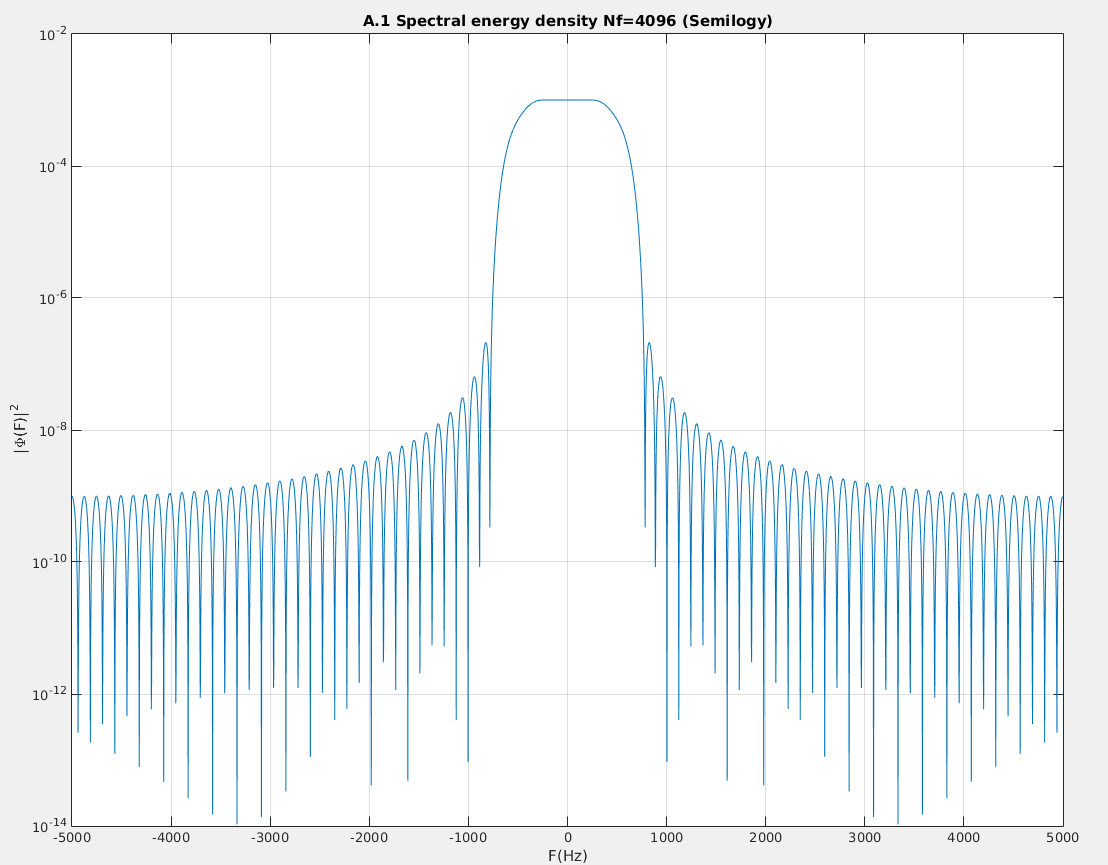
\includegraphics[scale=0.5, width=0.8\textwidth]{figures/A1-SED.png} \\
        \caption{A.1 Spectral Energy Density of \phi(t)}
    \end{figure}
    
    \begin{lstlisting}[caption = {A.1 Create SRRC pulse and display SED}]
T=10^-3 ; over=10 ; Ts=T/over ; A=4 ; a=0.5 ; Nf = 4096 ; Fs = 1/Ts ; 

[phi_t, t_phi] = srrc_pulse(T, Ts, A, a);           % Create SRRC pulse  
[Phi_F, F_Phi] = fourier_transform(phi_t, Ts, Nf);

% Display Spectral energy density of phi(t)
f=figure(); semilogy(F_Phi, abs(Phi_F).^2); grid on; 
    \end{lstlisting}

    %-------------------------------------
    %   A.2 subsection
    \subsection*{A.2 Create X(t) and calculate SDP}
    Όπως και για τον Fourier Transform παραπάνω, έτσι και για την δημιουργία του $X(t)$ υλοποιήθηκε μία συνάρτηση η οποία θα το δημιουργεί ακριβώς με τον τρόπο που αναφέρθηκε αναλυτικά στην πρώτη άσκηση. Από την στιγμή που στην συνέχεια της υλοποίησης χρησιμοποιείται και symbol mapping 4-PAM συνυπολογίζεται και αυτό στις παραμέτρους εισόδου της, ώστε να δημιουργεί κατάλληλα την $X(t)$ και για αυτή την περίπτωση. 
    Συγκεκριμένα αυτό που κάνει, είναι αρχικά να δημιουργεί την τυχαία ακολουθία από bit. 
    Έπειτα ανάλογα με το symbol mapping που επιλέχθηκε να δημιουργεί τα σύμβολα $X_n$. Για τον υπολογισμό του $X(t)$ ουσιαστικά όπως είδαμε και στην πρώτη άσκηση πρέπει να υπολογίσουμε την συνέλιξη με το υπερδειγματοληπτημένο σήμα $X_{\delta}$.
    Άρα ισχύει ότι $X(t) = \sum_{n=0}^{N-1}X_n\phi(t-nT) = X_δ (t) \circledast  φ(t)$. 
    Ενώ για να μπορέσουμε να καλύψουμε στην συνέχεια και τις απαιτήσεις του ερωτήματος Α.5 στο οποίο αλλάζουμε τις τιμές της περιόδου συμβόλου T και της τιμής του over, συμπεριλαμβάνονται και αυτά ως ορίσματα εισόδου της συνάρτησης.
    Σημαντικό σημείο είναι επίσης να προσέξουμε το διάστημα χρόνου για το $X_{\delta}$ μέχρι που θα εκτείνεται ο χρόνος, πράγμα το οποίο εξαρτάται από τον αριθμό των συμβόλων. 
    Τελευταίο πράγμα που υπολογίζει αυτή η συνάρτηση είναι η θεωρητική φασματική πυκνότητα ισχύος του σήματος που μόλις δημιουργήσαμε και θα χρησιμοποιηθεί στην συνέχεια ως μέτρο σύγκρισης με τα πειράματα. 
    Ο τρόπος με τον οποίο υπολογίζεται είναι με τον τύπο που εμφανίζεται και στην εκφώνηση $S_x(F)=\frac{σ_χ^2}{T}|\Phi{F}|^2$, προσέχοντας ότι το $σ_χ^2$ μπορούμε να το υπολογίσουμε είτε αμέσως ανάλογα με το symbol mapping (2-PAM: $σ_χ^2=\frac{(-1)^2+(1)^2}{2}$, 4-PAM: $σ_χ^2=\frac{(-3)^2+(-1)^2+(1)^2+(3)^2)}{4}$) - πράγμα που επιλέχθηκε αφού είναι θεωρητική προσέγγιση - είτε να χρησιμοποιήσουμε την συνάρτηση var έχοντας τα ίδια αποτελέσματα.
    Χρησιμοποιώντας λοιπόν αυτήν την συνάρτηση μπορούμε να δημιουργήσουμε πολλαπλά $X(t)$ σήματα πολύ εύκολα και γρήγορα.
    Για την \emph{\texttt{bits\_to\_2PAM.m}} αναφέρθηκε στην πρώτη άσκηση η υλοποίηση της, ενώ για την \emph{\texttt{bits\_to\_4PAM.m}} θα δοθεί στο ερώτημα Α.4.
    
    \begin{lstlisting}[caption = {\texttt{create\_xt.m}}]
function [Xt, t_Xt, T_PSD] = create_xt(part, N, PAM, phi_t, t_phi, Phi_F, Ts, T, over, DEBUG)
    
    % Create bits
    b=(sign(randn(N, 1)) + 1)/2; 

    if (PAM == 2)
        Xn = bits_to_2PAM(b);                   % Create symbols 
        X_delta = 1/Ts * upsample(Xn, over);    % Create upsampled X_delta signal              
        t_delta = [ 0 : Ts : (N*over-1)*Ts ];
    elseif (PAM == 4)
        Xn = bits_to_4PAM(b);                    % Create symbols
        X_delta = 1/Ts * upsample(Xn, over);     % Create upsampled X_delta signal            
        t_delta = [ 0 : Ts : ((N/2)*over-1)*Ts ];
    else
        disp('Not supported value of N-PAM encoding')
        return
    end
    
    % Calculate X_t, which is the convolution of phi(t) and X_delta
    Xt = conv(X_delta, phi_t).*Ts;
    t_Xt = [t_delta(1) + t_phi(1) : Ts : t_delta(end) + t_phi(end)];
    
    % Calculate theoretical PSD
    if (PAM == 2)
        var_Xn = ((-1)^2+(1)^2)./2;
        T_PSD = (var_Xn/T).*(abs(Phi_F).^2);
    elseif(PAM == 4)
        var_Xn = ((-3)^2 + (-1)^2 + (1)^2 + (3)^2)./4;
        T_PSD = (var_Xn/T).*(abs(Phi_F).^2);
    end
end
    \end{lstlisting}
    
    \par \noindent
    Έχοντας αναφέρει τα παραπάνω μπορούμε πλέον πολύ εύκολα για τις ανάγκες του ερωτήματος να δημιου- ργήσουμε την συνάρτηση $X(t)$ για $Ν=100$ και με χρήση $2-PAM$ symbol mapping, με τον παρακάτω τρόπο:
    
    \begin{lstlisting}[caption = {\texttt{Α.2 Create X(t)}}]
N=100 ; PAM = 2 ;
[Xt, t_Xt, Sx_F] = create_xt('A.2', N, PAM, phi_t, t_phi, Phi_F, Ts, T, over, 'T');  
    \end{lstlisting}
    
    \par \noindent
    Να σημειωθεί ότι υπάρχει ένα ακόμα χωρίο κώδικα μέσα στην συνάρτηση το οποίο εάν είναι ενεργοποιημένο το DEBUG mode (με το πέρασμα της τιμής `Τ' για την παράμετρο DEBUG) να μας εμφανίσει κατάλληλα τα δημιουργημένα σήματα (την ακολουθία bits, τα σύμβολα Xn και το σήμα X(t)). 
    
    \begin{figure}[H]
        \centering
        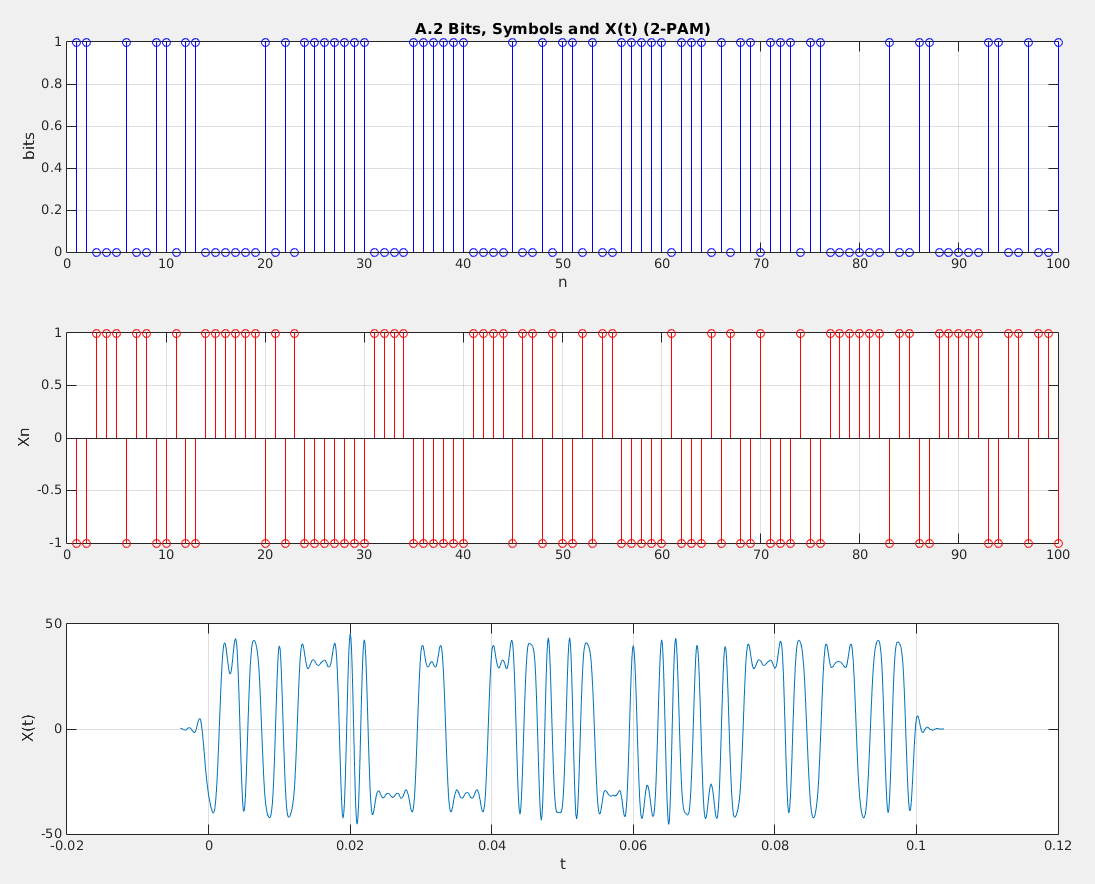
\includegraphics[scale=0.5, width=\textwidth]{figures/A2-b_Xn_Xt.png} \\
        \caption{A.2 Display bits, Xn and X(t) - 2-PAM}
    \end{figure}
    
    
    %-------------------------------------
    %   A.3 subsection
    \subsection*{A.3 Periodogram - Theoretical and Experimental PSD}
    Αρχικά πρώτο ζητούμενο είναι να υπολογιστεί το περιοδόγραμμα της X(t). 
    Εδώ είναι και ένα ενδιαφέρον σημείο διότι είναι το πρώτο σημείο στο οποίο δημιουργήθηκε μία συνάρτηση και επαναχρησιμοποιήθηκε κώδικας καλώντας απλά άλλη συνάρτηση μέσα σε αυτή. 
    Συγκεκριμένα δημιουργήθηκε η συνάρτηση \emph{\texttt{periodogram.m}} η οποία εμφανίζεται παρακάτω και υπολογίζει τον Fourier Transform και έπειτα με την χρήση αυτού και της εφαρμογής του τύπου της εκφώνησης $P_X(F) = \frac{|F[X(t)]^2}{T_{total}}$ υπολογίζει την ζητούμενη πληροφορία. 
    Το σημείο το οποίο πρέπει να προσέξουμε είναι ότι το $T_{total}$  είναι ο συνολικός χρόνος διάρκειας της $X(t)$. 
    Άρα το γινόμενο του πλήθους των δειγμάτων επί την διάρκεια κάθε δείγματος.
    
    \begin{lstlisting}[caption = {periodogram.m}]
function [Px_F, F_Px] = periodogram(Xt, t_Xt, Ts, Nf)
    Ttotal = length(t_Xt)*Ts;
    [X_F, F_Px] = fourier_transform(Xt, Ts, Nf);
    Px_F = (abs(X_F).^2)./Ttotal;
end
    \end{lstlisting}

    \par \noindent
    Επειδή όμως η βασική δομή του ερωτήματος Α.3 εμφανίζεται με παρόμοιο τρόπο και στα επόμενα ερωτήματα δημιουργήθηκε η παρακάτω συνάρτηση η οποία υλοποιεί όλες τις απαραίτητες ενέργειες. 
    Ξεκινώντας δημιουργεί έναν SRRC pulse (ο λόγος που δεν περάστηκε ως όρισμα είναι για να μπορεί να χρησιμοποιηθεί εύκολα και για το ερώτημα Α.5 όπου χρειάζεται διαφορετικές τιμές Τ και over).
    Έπειτα υπολογίζεται το σήμα $X(t)$ όπως περιγράφηκε στο ερώτημα Α.2. και στην συνέχεια υπολογίζει το ζητούμενο περιοδόγραμμα. 
    Ενώ τέλος εκτελεί πειραματικά μία επαναλαμβανόμενη δημιουργία $X(t)$ σημάτων προκειμένου να υπολογίσει τις αριθμητικές μέσες τιμές (με την χρήση του mean) των περιδογραμμάτων αυτών. 
    Σαν αποτέλεσμα μετά από αυτήν την διαδικασία θα έχουμε τόσο την θεωρητική φασματική πυκνότητα ισχύος όσο και την πειραματική.  
    Να ξανά γίνει αναφορά ότι παρόλο που μέσα σε αυτήν την συνάρτηση εμφανίζονται τα ζητούμενα σήματα ΜΟΝΟ όταν ζητείται το καθένα (γίνονται κάποιοι έλεγχοι σχετικά με ορίσματα \emph{\texttt{partA}} για το περιοδόγραμμα και \emph{\texttt{partΒ}} για το PSD, αν είναι κενό το εκάστοτε πεδίο τότε δεν εμφανίζεται το ανάλογο σήμα) αυτό δεν εμφανίζεται εδώ - υπάρχει στο τέλος όμως - ώστε να δοθεί προσοχή μόνο στους υπολογισμούς.
    \par \noindent
    \textbf{Σημείωση:} Από την στιγμή που αναφέρεται να δοθεί το περιοδόγραμμα μίας υλοποίησης της $X(t)$ και όχι να είναι η ίδια κατά μήκος των `συ-σχετιζόμενων' ερωτημάτων δεν μας πειράζει που δημιουργούνται από την αρχή σε κάθε ερώτημα με διαφορετικά bit καθώς θεωρείται ότι αναλύεται από την θεωρητική όψη.
    
    % Είναι σημαντικό να ξανά σημειωθεί ότι κομμάτια σχετικά με την εμφάνιση των σημάτων δεν εμφανίζονται εδώ, αλλά πρέπει να αναφερθεί ότι τα ορίσματα \emph{\texttt{partA}} και \emph{\texttt{partB}} συσχετίζονται με την εμφάνιση του periogram και του PSD και αν ένα από τα δύο είναι άδειο αυτό σημαίνει ότι δεν χρειαζόμαστε να εμφανίσουμε διάγραμμα για αυτό. 
    
    \begin{lstlisting}[caption = {\texttt{display\_periodogram\_PSD\_theoretical\_experimental.m}}]
function [periodogram_figure, theoritical_practical_PSD_figure] = display_periodogram_PSD_theoretical_experimental(partA, partB, PAM, T, Ts, A, a, Nf, N, K, over)
    
 [phi_t, t_phi] = srrc_pulse(T, Ts, A, a);           % Create SRRC pulse  
 [Phi_F, F_Phi] = fourier_transform(phi_t, Ts, Nf);
 [Xt, t_Xt, Sx_F] = create_xt(partA, N, PAM, phi_t, t_phi, Phi_F, Ts, T, over, DEBUG);
 [Px_F, F_Px] = periodogram(Xt, t_Xt, Ts, Nf);
    
 % Experimental PSD 
 for i = 1:K                                            
    [Xt, t_Xt] = create_xt('', N, PAM, phi_t, t_phi, Phi_F, Ts, T, over, 'F');
    Px_experiments(i,:) = periodogram(Xt, t_Xt, Ts, Nf);
 end
    
 Px_F_experimental = mean(Px_experiments);           
 Px_F_theoritical = Sx_F;                        	
end
    \end{lstlisting}
    
    \par \noindent
    Έχοντας κάνει όλα τα παραπάνω, τελικά για τον υπολογισμό όλου του ερωτήματος Α.3 το μόνο που έχουμε να κάνουμε είναι να εκτελέσουμε τις παρακάτω γραμμές κώδικα.
    Καλώντας την \texttt{display\_periodogram\_PSD \_theoretical\_experimental.m} υπολογίζονται λοιπόν τα δύο πρώτα υπό-ερωτήματα ενώ στην συνέχεια δοκιμάζουμε διαφορετικές τιμές Ν κι Κ για να απαντήσουμε στο τρίτο υποερώτημα.
    
    \begin{lstlisting}[caption = {A.3 Periodogram - theoretical and practical PSD}]
K=100; PAM = 2;
display_periodogram_PSD_theoretical_experimental('A.3.a', 'A.3.b', PAM, T, Ts, A, a, Nf, N, K, over)
for Ni = [5 10 30 50 100] 
    for Ki = [5 10 30 50 100]
        display_periodogram_PSD_theoretical_experimental('', 'A.3.c', PAM, T, Ts, A, a, Nf, Ni, Ki, over)
    end
end
    \end{lstlisting}
    
      \begin{figure}[H]
        \centering
        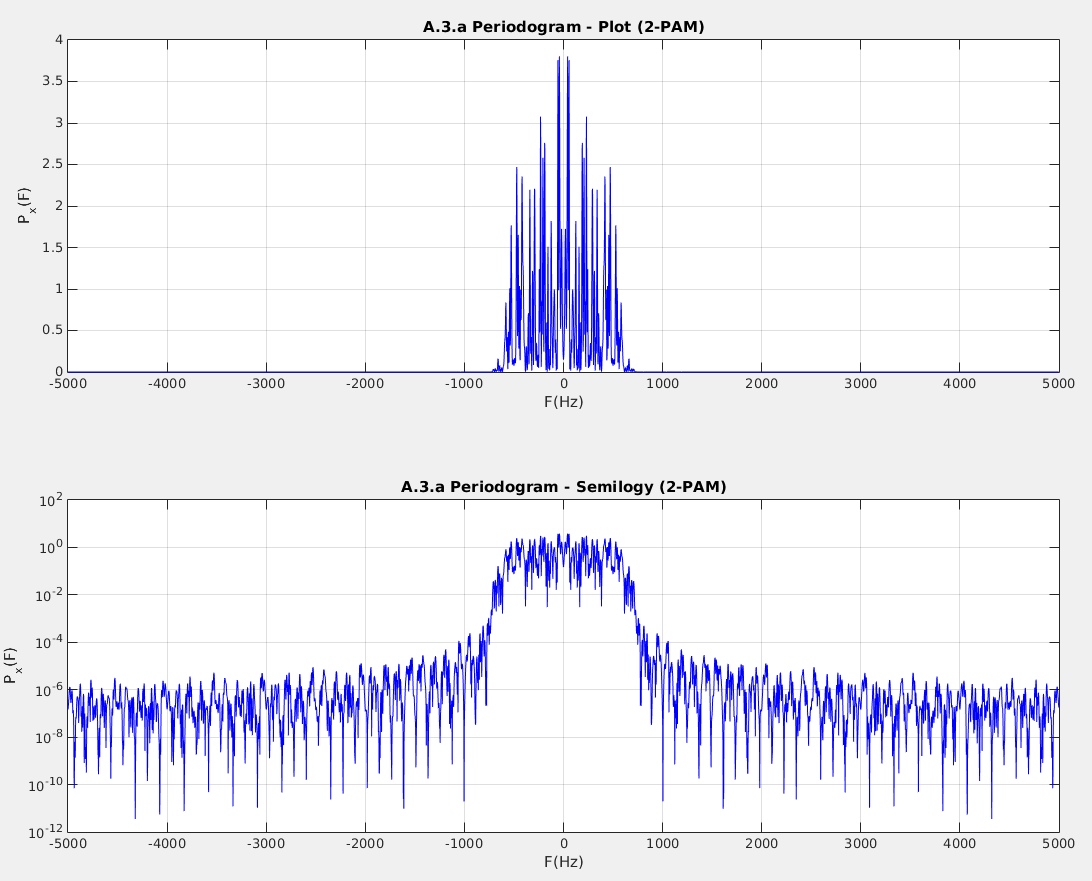
\includegraphics[scale=0.5, width=0.8\textwidth]{figures/A3.1-Periodogram.png} \\
        \caption{A.3.a Περιοδόγραμμα μίας υλοποίησης X(t) (2-PAM) σε plot και semilogy}
    \end{figure}
    
      \begin{figure}[H]
        \centering
        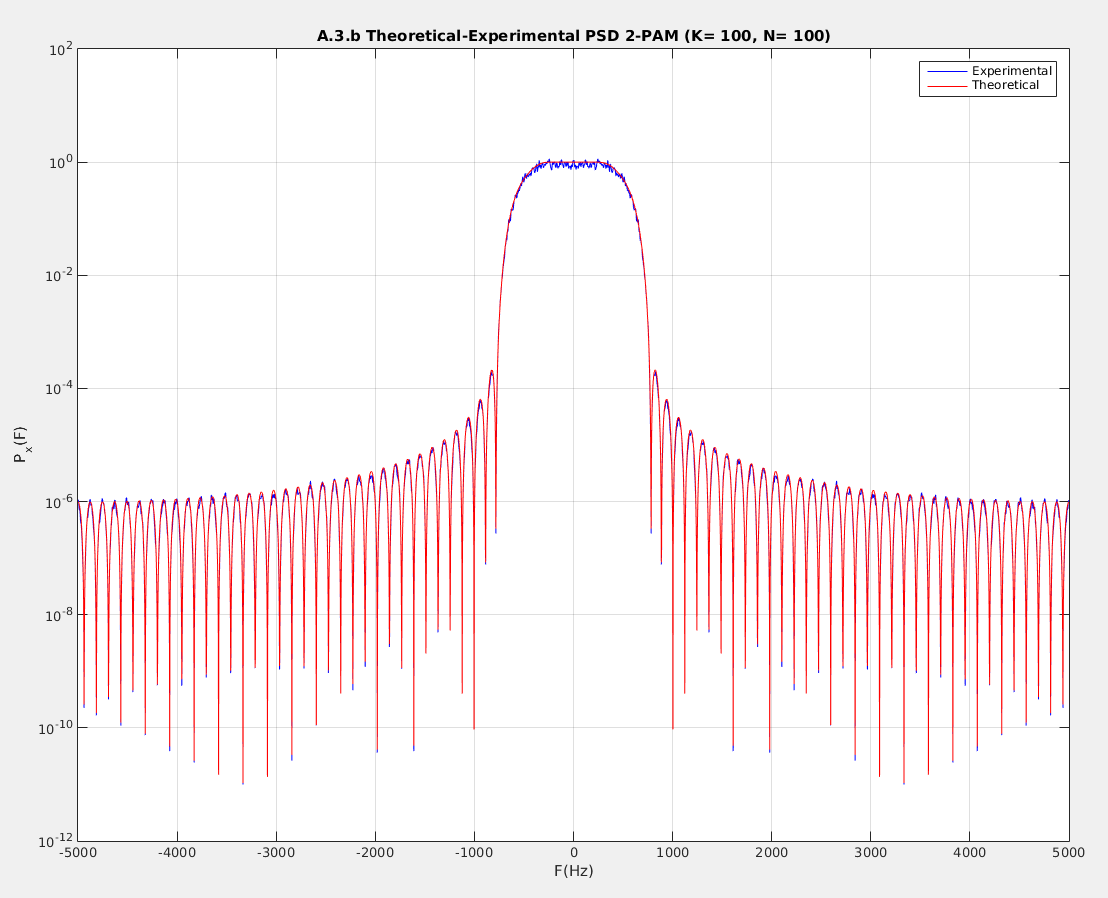
\includegraphics[scale=0.5, width=0.8\textwidth]{figures/A3.2-T_E_PSD.png} \\
        \caption{A.3.b Πειραματική και Θεωρητική φασματική πυκνότητα ισχύος σε κοινό semilogy}
    \end{figure}
    
    \par \noindent
    Δεν δίνονται figures για το τρίτο υπο-ερώτημα στο οποίο επαναλαμβάνουμε το πείραμα για διαφορετικές τιμές Ν και Κ αλλά αυτό που μπορούμε να παρατηρήσουμε είναι ότι.
    Καθώς αυξάνεται το Ν το αποτέλεσμα τείνει να ταυτιστεί με το θεωρητικό, ενώ όσο αυξάνεται το Κ τόσο καλύτερη γίνεται και η προσέγγιση.
    Ο λόγος είναι ότι όντας το περιοδόγραμμα ένα στιγμιότυπο της PSD μετά από ένα αριθμό επαναλήψεων είναι αρκετά κοντά να συνθέσει την ιδανική και θεωρητική PSD.
    Μετά όμως από ένα σημείο τιμών δεν παρατηρούνται περισσότερες αλλαγές.
    
    %-------------------------------------
    %   A.4 subsection
    \subsection*{A.4 X(t) - 4-PAM }
    Πρώτο κομμάτι του συγκεκριμένου ερωτήματος ήταν η δημιουργία μίας συνάρτησης η οποία θα κάνει την ζητούμενη απεικόνιση συμβόλων 4-PAM.
    Παρακάτω παρουσιάζεται η συνάρτηση που δημιουργήθηκε ακολουθώντας απλές συνθήκες ελέγχου.
    
    \begin{lstlisting}[caption = {\emph{\texttt{bits\_to\_4PAM.m}}}]
function [ Xout ] = bits_to_4PAM( X )
    if(mod(length(X),2)==1)
        Xout=[0];
    else
        i=1;
        while i<=length(X)
            b1=X(i);b2=X(i+1);
 
            if(b1==0 && b2==0)
               temp(i)=3; 
            elseif(b1==0 && b2==1)
               temp(i)=1;
            elseif(b1==1 && b2==1)
               temp(i)=-1; 
            elseif(b1==1 && b2==0)
               temp(i)=-3;      
            end
            i=i+2;
            Xout=temp(temp~=0);
        end
    end
end
    \end{lstlisting}
    
    \par \noindent
    Για την απάντηση του πρώτου υπό-ερωτήματος αρκεί να ανατρέξουμε στην βασική συνάρτηση που αναλύσαμε στο Α.3 ερώτημα σκεπτόμενοι την ανάλυση για την δημιουργία του X(t) που έγινε στο Α.2 ερώτημα.
    Ενώ εκτός από τα ζητούμενα δύο διαγράμματα εμφανίζονται όπως και στο A.2 ερώτημα τα ενδιάμεσα σήματα που έγιναν προκειμένου να επαληθεύσουμε το X(t).
    
    \begin{lstlisting}[caption = {A.4.a Periodogram - Theoretical and Experimental PSD}]
PAM = 4;
display_periodogram_PSD_theoretical_experimental('A.4.a', 'A.4.a', PAM, T, Ts, A, a, Nf, N, K, over)
    \end{lstlisting}
    
    \begin{figure}[H]
        \centering
        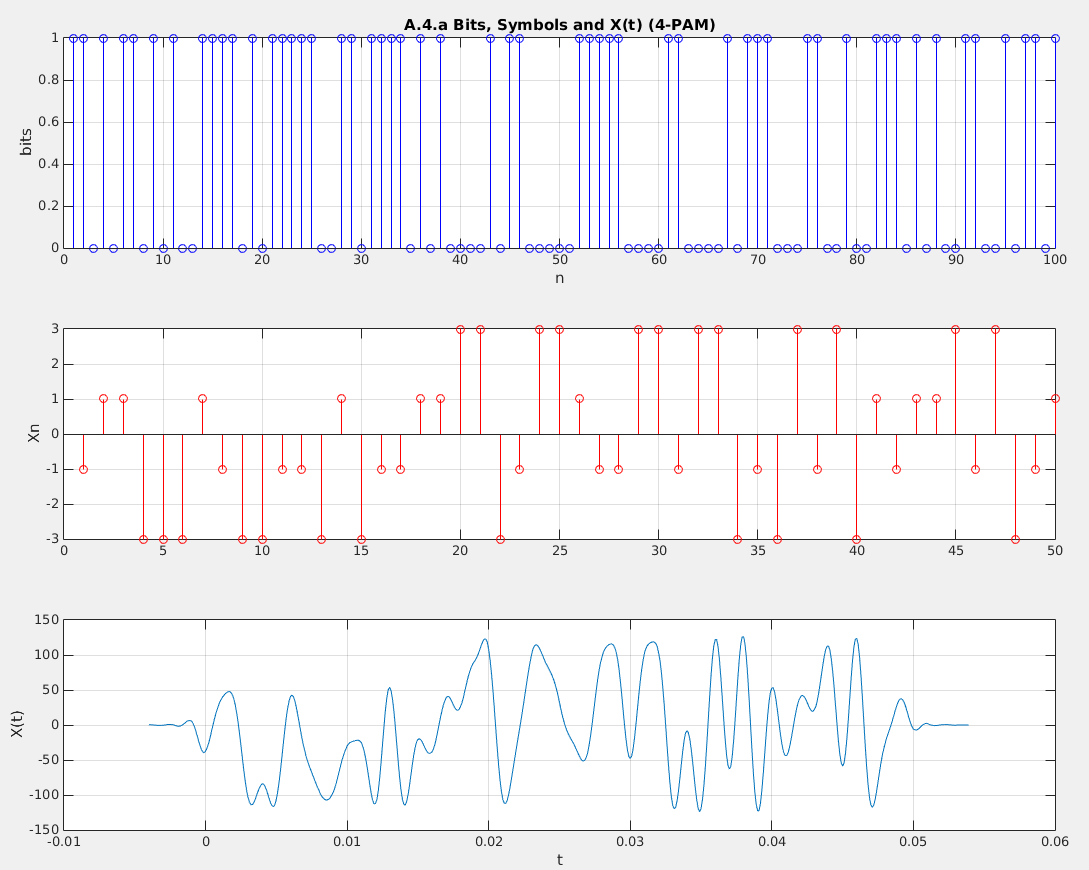
\includegraphics[scale=0.5, width=0.8\textwidth]{figures/A4.0-b_Xn_Xt.png} \\
        \caption{A.4 Display bit, Xn and X(t) - 4-PAM}
    \end{figure}
    
    \begin{figure}[H]
        \centering
        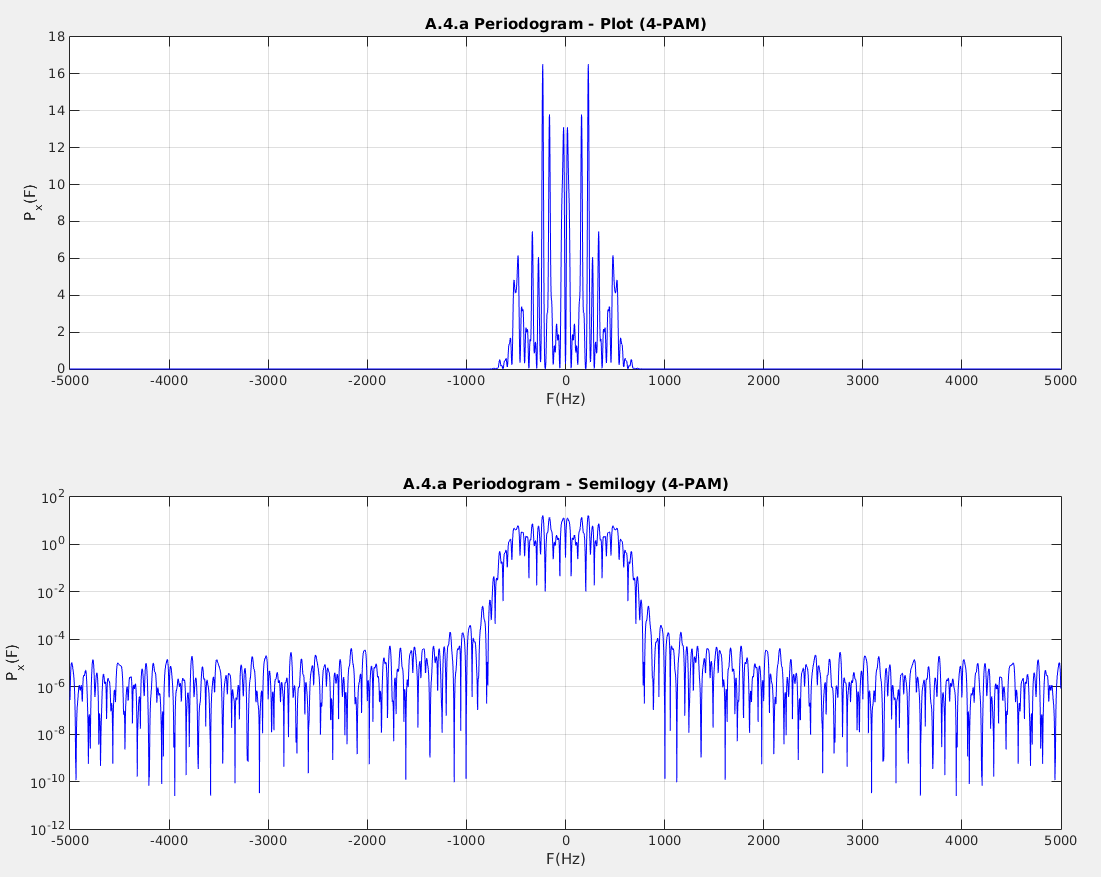
\includegraphics[scale=0.5, width=0.8\textwidth]{figures/A4.1-Periodogram.png} \\
        \caption{A.4.a Περιοδόγραμμα μίας υλοποίησης X(t) (4-PAM) σε plot και semilogy}
    \end{figure}
    
      \begin{figure}[H]
        \centering
        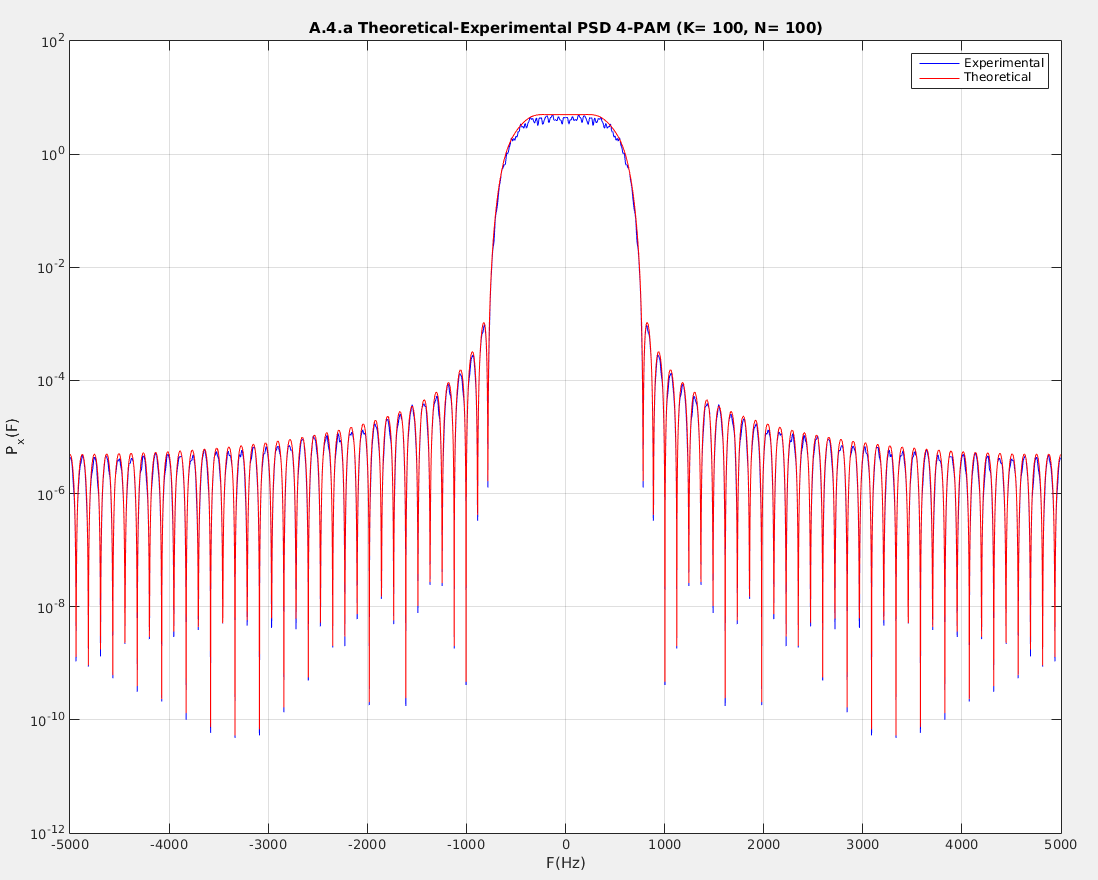
\includegraphics[scale=0.5, width=0.8\textwidth]{figures/A4.1-T_E_PSD.png} \\
        \caption{A.4.a Πειραματική και Θεωρητική φασματική πυκνότητα ισχύος σε κοινό semilogy}
    \end{figure}
    
    
    \par \noindent
    Σχετικά με το δεύτερο υπό-ερώτημα αυτό που μπορούμε να παρατηρήσουμε είναι ότι και στις δύο περιπτώσεις (με χρήση 2-PAM vs 4-PAM) το εύρος φάσματος της PSD τους είναι το ίδιο.
    Πράγμα λογικό καθώς το θεωρητικό εύρος φάσματος των παλμών άπειρης διάρκειας είναι $BW=\frac{1+a}{2T}$, άρα δεν θα έπρεπε να διαφέρει.
    Δεν μπορούμε όμως να πούμε ότι ισχύει αυτό και για το μέγιστο πλάτος των PSD, καθώς η 4-PAM έχει μεγαλύτερο πλάτος πράγμα το οποίο συμβαίνει λόγο του symbol mapping της.
    
    
    
    %-------------------------------------
    %   A.5 subsection
    \subsection*{A.5 Επανάληψη του Α.3 για διαφορετικό T}
    Και σε αυτό το ερώτημα εξαιτίας της συνάρτησης που δημιουργήθηκε στο Α.3, είναι εύκολη η δημιουργία των κυμματομορφών.
    Σημαντικό σημείο είναι ότι αφού ζητείται να κρατηθεί ίδια περίοδος δειγματοληψίας έπρεπε να διπλασιαστεί επίσης η παράμετρος over. 
    Άρα για την υλοποίηση του πρώτου υπό-ερωτήματος, έπρεπε να εκτελέσουμε το παρακάτω κομμάτι κώδικα. Όπου αρχικά δημιουργούμε το περιοδόγραμμα της X(t), μετά συγκρίνουμε το θεωρητικό με το πειραματικό PSD και τέλος επαναλαμβάνουμε για διαφορετικές τιμές Κ και Ν:
    
    \begin{lstlisting}[caption = {A.5 Επανάληψη του Α.3 για διαφορετικό T}]
PAM=2;
display_periodogram_PSD_theoretical_experimental('A.5.a', 'A.5.a', PAM, 2*T, Ts, A, a, Nf, N, K, 2*over)

for Ni = [5 10 30 50 100] 
    for Ki = [5 10 30 50 100]
        display_periodogram_PSD_theoretical_experimental('', 'A.5.c', PAM, 2*T, Ts, A, a, Nf, Ni, Ki, 2*over)
    end
end
    \end{lstlisting}
    
      \begin{figure}[H]
        \centering
        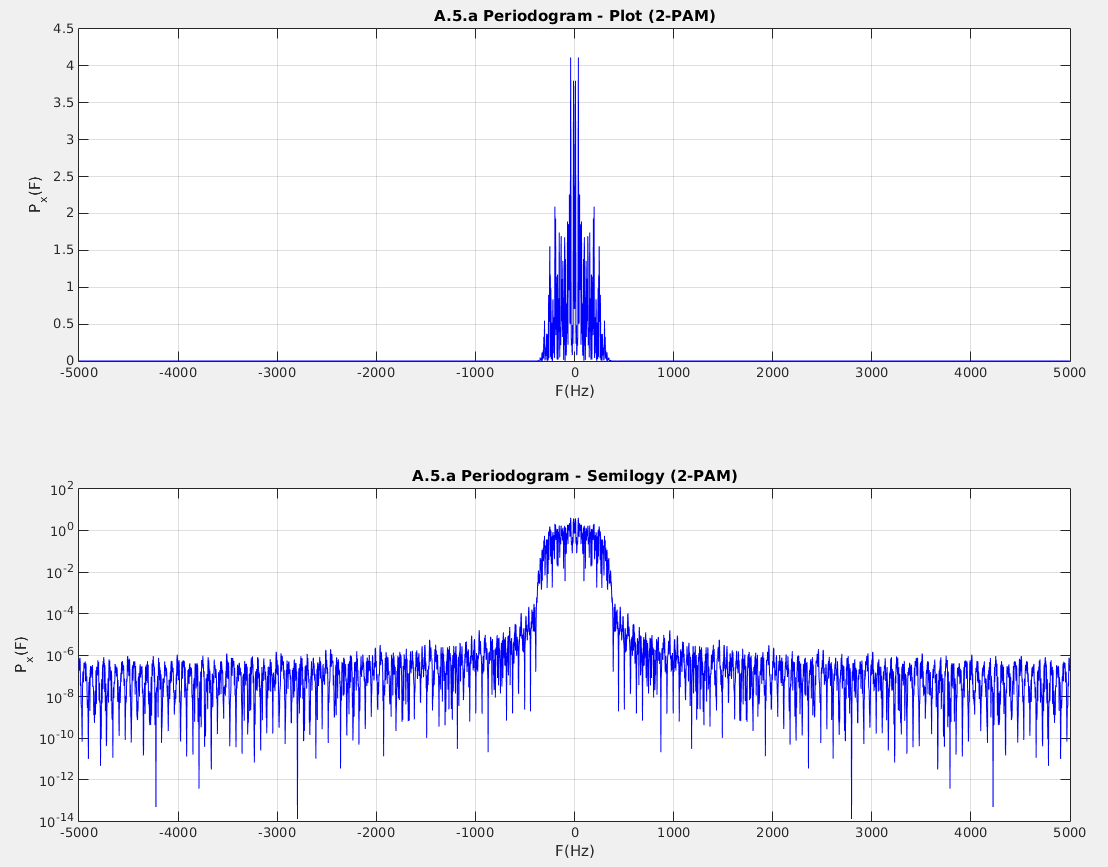
\includegraphics[scale=0.5, width=0.85\textwidth]{figures/A5.1-Periodogram.png} \\
        \caption{A.5.a T'=2T - Περιοδόγραμμα μίας υλοποίησης X(t) (2-PAM) σε plot και semilogy}
    \end{figure}
    
      \begin{figure}[H]
        \centering
        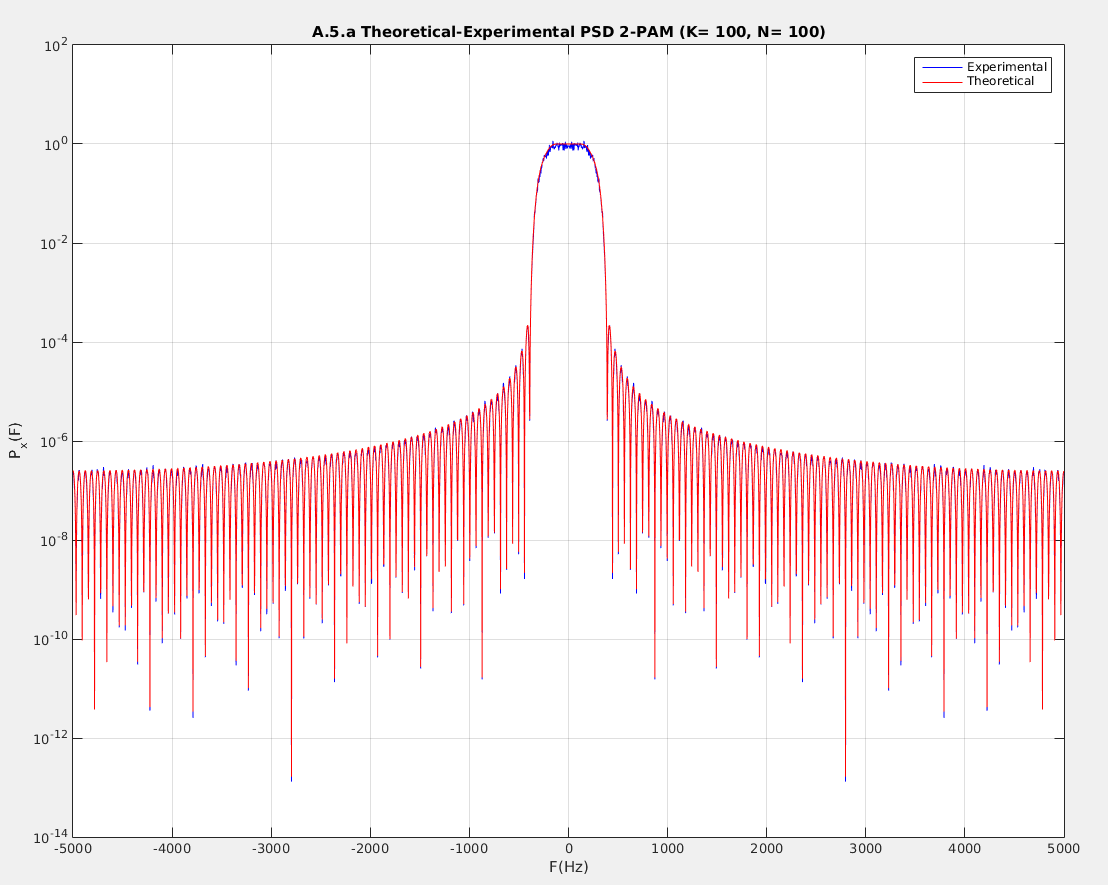
\includegraphics[scale=0.5, width=0.85\textwidth]{figures/A5.1-T_E_PSD.png} \\
        \caption{A.5.a T'=2T - Πειραματική και Θεωρητική φασματική πυκνότητα ισχύος σε κοινό semilogy}
    \end{figure}
    
    
    \par \noindent
    Σε αντίθεση με το Α.4, σε αυτό το ερώτημα αν συγκρίνουμε το εύρος φάσματος της PSD του Α.3 ερωτήματος με του Α.5 θα δούμε ότι διαφέρουν. 
    Συγκεκριμένα στο Α.5 παρατηρούμε ότι υπάρχει υπο-διπλασιασμός του εύρους φάσματος το οποίο όπως αναφέραμε παραπάνω είναι λογικό καθώς το θεωρητικό εύρος φάσματος των παλμών άπειρης διάρκειας είναι $BW=\frac{1+a}{2T}$. Άρα για διπλάσια περίοδο συμβόλου Τ με σταθερό α, θα έχουμε υπο-διπλασιασμό του Bandwidth.
    
    %-------------------------------------
    %   A.6 subsection
    \subsection*{A.6 2-PAM vs 4-PAM}
    a) Συγκρίνοντας την ταχύτητα επικοινωνίας με χρήση κωδικοποιήσεων 2-PAM versus 4-PAM για ίδιο εύρος φάσματος έχουμε το εξής. 
    Κατά την επικοινωνία με 2-PAM στέλνονται $log_2 2=1$bit πληροφορίας καθώς κάθε σύμβολο κωδικοποιεί ακριβώς 1 bit.
    Αντίθετα για επικοινωνία με 4-PAM έχουμε αποστολή $log_2 4 =2$bits καθώς κάθε σύμβολο κωδικοποιεί 2 bits πληροφορίας.
    Συνεπώς με την 4-PAM μεταφέρονται περισσότερα bits per symbol άρα και ταχύτερη μετάδοση δεδομένων στο ίδιο bandwidth. 
    Αυτό όμως δεν σημαίνει ότι δεν υπάρχουν μειονεκτήματα.
    Όσο περισσότερα bits πληροφορίας περιέχει κάθε σύμβολο τόσο πιο πολύπλοκη γίνεται η κωδικοποίηση/αποκωδικοποίηση της.
    Άρα παρά το πλεονέκτημα στην ταχύτητα, απαιτείται περισσότερη επεξεργαστική ισχύς ενώ παράλληλα αυξάνεται και το SNR προκειμένου να διατηρηθεί το ίδιο bit-error-rate. 
    
    \par \noindent
    b) Αν είχαμε να επιλέξουμε περίοδο συμβόλου μεταξύ μίας υλοποίησης με Τ και μίας άλλης με Τ'=2Τ σε ένα πολύ ακριβό εύρος φάσματος, αυτό που θα επιλέγαμε είναι το Τ'. 
    Ο λόγος είναι - και τα σχεδιαγράμματα από τα ερωτήματα Α.3 και Α.5 το επαληθεύουν - ότι για διπλάσιο Τ το Bandwidth περιορίζεται στο μισό, αυξάνοντας παράλληλα και την απαιτούμενη ενέργεια επιτυχούς μετάδοσης.
    
    
    
    %-------------------------------------------------------------------------
    %   B section
    \section*{Ερώτημα B}
    Έχουμε την ακολουθία ανεξάρτητων Συμβόλων $X_n$
    
    \[ X(t) = \sum_{n=-\infty}^{\infty} Xn\phi(t-nT) \]
    
    \par \noindent
    Όπου $\mathcal{E}[X_n]=0, \mathcal{E}[X_n^2]=\sigma_x^2$ και $T>0$. Επιπλέον έχουμε το διαμορφωμένο σήμα $Y(t) = X(t)\cos(2 \pi f_o + \Theta)$, όπου Θ τυχαία μεταβλητή ομοιόμορφα κατανεμημένη στο $[0,2\pi)$ ανεξάρτητη των $X_n$ για κάθε n. Επίσης ΣΠΠ της Θ:
    
    \[  
        F_{\Theta}(\theta) = \left\{ 
                    \begin{array}{rcl}
                        \frac{1}{2\pi}, & 0 \leq \theta \leq 2\pi \\ 
                        0,  & \text{αλλού}
                    \end{array}
                \right.
    \]
    
    %-------------------------------------
    %   B.1 subsection
    \subsection*{B.1}
    α)
    \begin{align}
        \mathcal{E}[Y(t)] &= \mathcal{E}[X(t)\cos(2 \pi f_o + \Theta)] \overset{indep.}{=} \mathcal{E}[X(t)] \mathcal{E}[\cos(2 \pi f_o + \Theta)] \nonumber \\
        &= \mathcal{E}[X(t)] \int_{-\infty}^{\infty} \cos (2\pi f_o t + \Theta) F_{\Theta}(\Theta)d\theta \nonumber \\
        &= \mathcal{E}[X(t)] \int_{0}^{2\pi} \cos (2\pi f_o t + \Theta) \frac{1}{2\pi} d\theta \nonumber \\
        &= \frac{1}{2\pi}  \mathcal{E}[X(t)] \int_{0}^{2\pi} \cancelto{0}{\cos (2\pi f_o t + \Theta) d\theta} \nonumber \\
        &= \boxed{0} \text{, \spaceΆρα σταθερή}
    \end{align}
    
    \par \noindent
    %----------------------
    β) Γνωρίζοντας την παρακάτω σχέση:
    \begin{align}
        \cos a \cos b = \frac{1}{2}[\cos(a+b) \ + \cos(a-b)] \label{cosa-cosb}
    \end{align}
    
    \begin{align}
        \mathcal{E}[Y(t+\tau)Y(t)] = R_{yy}(t+\tau,t) =& \mathcal{E} [X( t + \tau) \cos(2 \pi f_0 (t + \tau) + \Theta) X(t) \cos(2 \pi f_0 t + \Theta)] \nonumber \\
        \overset{indep.}{=}& \mathcal{E}[X(t+\tau)X(t)] \mathcal{E}[\cos(2\pi f_0(t+\tau) +\Theta)\cos(2\pi f_0t + \Theta)] \nonumber \\
        \overset{(\ref{cosa-cosb})}{=}& \mathcal{E}[X(t+\tau)X(t)]\frac{1}{2}\mathcal{E}[\cancelto{0}{\cos(4\pi f_0t+2\pi f_0\tau+2\Theta)} + \cos(2\pi f_0\tau)] \nonumber \\
        =& \frac{1}{2} \mathcal{E}[X(t+\tau)X(t)] \cos(2\pi f_0\tau) \nonumber \\ 
        =& \boxed{ \frac{1}{2} R_{xx}(t+\tau,t)\cos(2\pi f_0\tau)}
    \end{align}
    
    %-------------------------------------
    %   B.2 subsection
    \subsection*{B.2}
    Μία στοχαστική διαδικασία Y(t) καλείται κυκλοστάσιμη υπό την ευρεία έννοια με περίοδο T αν:
    
    \begin{enumerate}
      \item $m_Y (t) = m_Y (t + T )$, \space $\forall t \in \mathbb{R}$
      \item $R_{YY} (t + τ, t) = R_{YY} (t + T + τ, t + T )$, \space $\forall t \in \mathbb{R}$
    \end{enumerate}

    \par \noindent
    Το πρώτο το είδαμε παραπάνω οπότε ελέγχουμε την $R_{xx}(t+\tau,t)$ ως προς τη περιοδικότητα.
    
    \begin{align}
        R_{xx}(t+\tau,t) &= \mathcal{E}[X(t+\tau)X(t)] \nonumber \\
        &= \mathcal{E}\left[ \sum_{n=-\infty}^{\infty} X_n \phi(t+\tau-nT) \sum_{n=-\infty}^{\infty} X_n \phi(t-nT) \right] \nonumber \\
        &= \mathcal{E}\left[\sum_{n=-\infty}^{\infty} \sum_{n=-\infty}^{\infty} X_n^2 \phi(t+\tau-nT) \phi(t-nT)  \right] \nonumber \\
        &= \mathcal{E}\left[\ X_n^2 \right] \sum_{n=-\infty}^{\infty} \phi(t+\tau-nT) \phi(t-nT) \nonumber \\
        &\overset{given}{=} \boxed{ σ_χ^2 \sum_{n=-\infty}^{\infty} \phi(t+\tau-nT) \phi(t-nT)}  \Rightarrow \mbox{ κυκλοστάσιμη } \forall \mbox{ T} \label{R-xx} \\ 
        &= R_{xx}(t+\tau+T,t+T) \nonumber
    \end{align}
    
    \begin{align}
        \boxed{R_{yy}(t+\tau,t) = R_{xx}(t+\tau+T,t+T)\cos(2\pi f_0\tau) = R_{yy}(t+\tau+T,t+T)}
    \end{align}
    
    \par \noindent
    Άρα είναι περιοδική κυκλοστάστιμη υπό την ευρεία έννοια
    
    %-------------------------------------
    %   B.3 subsection
    \subsection*{B.3}
    Αφού Υ(t) κυκλοστάσιμη, υπό την ευρεία έννοια, με περίοδο T , τότε ξέρουμε ότι ισχύουν οι παρακάτω σχέσεις:
    
    \begin{itemize}
      \item $S_y(F) = \mathcal{F}\{\bar{R}_{y}(t)\} $
      \item $\bar{R}_{y}(t) = \frac{1}{T} \int_{T} R_{yy}(t + τ, t) dt$
    \end{itemize}
    
    \par \noindent
    Για το Χ έχουμε ότι:
    \begin{align}
        \bar{R}_{x}(t) &= \frac{1}{T} \int_{T} R_{xx} (t + τ, t) dt \nonumber \\
        &\overset{(\ref{R-xx})}{=} \frac{1}{T} \int_{T} σ_χ^2 \sum_{-\infty}^{\infty} \left[ \phi(t+\tau-nT) \phi(t-nT)  \right]  dt \nonumber \\
        &= \frac{σ_χ^2}{T}  \int_{T} \sum_{-\infty}^{\infty} \left[ \phi(t+\tau-nT) \phi(t-nT)  \right]  dt \nonumber \\
        &= \boxed{\frac{σ_χ^2}{T}  (\phi(\tau) + \phi(-\tau))} \label{Rx} 
    \end{align}
    
    \par \noindent
    Μέση αυτοσυσχέτιση της Y εντός μίας περιόδου ορίζουμε ως: 
    \begin{align}
        \bar{R}_{y}(t) &= \frac{1}{T} \int_{T} R_{yy} (t + τ, t) dt = \frac{1}{T} \int_{T} \frac{1}{2} R_{xx}(t+\tau,t) \cos(2\pi f_0\tau) dt \nonumber \\
        &\overset{(\ref{R-xx})}{=} \frac{1}{T} \int_{T} \frac{1}{2} σ_χ^2 \sum_{-\infty}^{\infty} \left[ \phi(t+\tau-nT) \phi(t-nT)  \right] \cos(2\pi f_0\tau) dt \nonumber \\
        &= \frac{σ_χ^2}{2T}  \int_{T} \sum_{-\infty}^{\infty} \left[ \phi(t+\tau-nT) \phi(t-nT)  \right] \cos(2\pi f_0\tau) dt \nonumber \\
        &= \frac{σ_χ^2}{2T} \cos(2\pi f_0\tau) (\phi(\tau) + \phi(-\tau)) \nonumber \\
        &\overset{(\ref{Rx})}{=} \boxed{\frac{1}{2}\bar{R}_{x}(t) \cos(2\pi f_0\tau)}
    \end{align}
    
    \par \noindent
    Μία από τις ιδιότητες του Fourier για μία συνάρτηση x(t) είναι η εξής:
    \begin{align}
        \mathcal{F}\{ x(t) \cos(2 \pi f_{o} t) \} = \frac{1}{2} \left[ X(F+f_{ο}) + X(F-f_{ο}) \right] \label{fourier-property}
    \end{align}
    
    \par \noindent
    Επίσης έχουμε $S_y(F) = \mathcal{F}\{\bar{R}_{y}(t)\} $. Άρα:
    \begin{align*}
        S_y(f_0) &= \mathcal{F}\{\bar{R}_{y}(t)\} = \mathcal{F}\{\frac{1}{2}\bar{R}_{x}(t) \cos(2\pi f_0\tau)\} \\
        &\overset{(\ref{fourier-property})}{=} \boxed{\frac{1}{4} \left[ S_x(F+f_0)  + S_x(F-f_0) \right]}
    \end{align*}
    
    \par \noindent
    Λογικό αποτέλεσμα καθώς το σήμα πολλαπλασιάζεται με περιοδικό σήμα το οποίο προκαλεί μετατόπιση βάση της συχνότητας $f_o$ και με trade-off το πλάτος του.
    
    %-------------------------------------
    %   B.4 subsection
    \subsection*{B.4}
    
    
%---------------------------------------------------------------------------------------------------------------
%
%   Codes
%
%
\newpage

\emph{Code:} \\
\rule{\linewidth}{0.3mm} \\[0.1cm]
%---------------------
\begin{lstlisting}[caption = {\texttt{bits\_to\_2PAM.m}}]
function [ Xo ] = bits_to_2PAM( Xi )
    Xo=zeros(1,length(Xi));    
    for i=1:length(Xi)    
        if(Xi(i)>0)          
            Xo(i)=-1;        
        else
            Xo(i)=1;    
        end
    end
end
\end{lstlisting}

%---------------------
\begin{lstlisting}[caption = {\texttt{bits\_to\_4PAM.m}}]
function [ Xout ] = bits_to_4PAM( X )
    if(mod(length(X),2)==1)
        Xout=[0];
    else
        i=1;
        while i<=length(X)
            b1=X(i);b2=X(i+1);
 
            if(b1==0 && b2==0)
               temp(i)=3; 
            elseif(b1==0 && b2==1)
               temp(i)=1;
            elseif(b1==1 && b2==1)
               temp(i)=-1; 
            elseif(b1==1 && b2==0)
               temp(i)=-3;      
            end
            i=i+2;
            Xout=temp(temp~=0);
        end
    end
end
\end{lstlisting}
\begin{lstlisting}[caption = {\texttt{fourier\_transform.m}}]
function [X_F, F_X] = fourier_transform(Xt, Ts, Nf)
    Fs = 1/Ts;
    X_F = fftshift(fft(Xt,Nf)*Ts);
    F_X = [-Fs/2 : Fs/Nf : Fs/2-Fs/Nf];
end
\end{lstlisting}

%---------------------
\begin{lstlisting}[caption = {\texttt{periodogram.m}}]
function [Px_F, F_Px] = periodogram(Xt, t_Xt, Ts, Nf)
    Ttotal = length(t_Xt)*Ts;
    [X_F, F_Px] = fourier_transform(Xt, Ts, Nf);
    Px_F = (abs(X_F).^2)./Ttotal;
end
\end{lstlisting}



%---------------------
\begin{lstlisting}[caption = {\texttt{create\_xt.m}}]
function [Xt, t_Xt, T_PSD] = create_xt(part, N, PAM, phi_t, t_phi, Phi_F, Ts, T, over, DEBUG)
    
    % Create bits
    b=(sign(randn(N, 1)) + 1)/2; 

    if (PAM == 2)
        Xn = bits_to_2PAM(b);                               % Create symbols 
        X_delta = 1/Ts * upsample(Xn, over);                % Create upsampled X_delta signal              
        t_delta = [ 0 : Ts : (N*over-1)*Ts ];
    elseif (PAM == 4)
        Xn = bits_to_4PAM(b);                               % Create symbols
        X_delta = 1/Ts * upsample(Xn, over);                % Create upsampled X_delta signal            
        t_delta = [ 0 : Ts : ((N/2)*over-1)*Ts ];
    else
        disp('Not supported value of N-PAM encoding')
        return
    end
    
    % Calculate X_t, which is the convolution of phi(t) and X_delta
    Xt = conv(X_delta, phi_t).*Ts;
    t_Xt = [t_delta(1) + t_phi(1) : Ts : t_delta(end) + t_phi(end)];
    
    % Only for debug display signals
    if (DEBUG == 'T'); figure(); subplot(3,1,1); stem([1:N],b,'b'); grid on; title(strcat(part, ' Bits, Symbols and X(t) (',num2str(PAM),'-PAM)')); ylabel('bits'); xlabel('n');if(PAM == 2);subplot(3,1,2) ; stem([1:N],Xn,'r'); grid on;ylabel('Xn'); elseif (PAM == 4);subplot(3,1,2) ; stem([1:N/2],Xn,'r'); grid on;ylabel('Xn'); end;subplot(3,1,3); plot(t_Xt,Xt); grid on;ylabel('X(t)'); xlabel('t');end
    
    % Calculate theoretical PSD
    if (PAM == 2)
        var_Xn = ((-1)^2+(1)^2)./2;
        T_PSD = (var_Xn/T).*(abs(Phi_F).^2);
    elseif(PAM == 4)
        var_Xn = ((-3)^2 + (-1)^2 + (1)^2 + (3)^2)./4;
        T_PSD = (var_Xn/T).*(abs(Phi_F).^2);
    end
end
\end{lstlisting}

%---------------------
\begin{lstlisting}[caption = {\texttt{display\_periodogram\_PSD\_theoretical\_experimental.m}}]
function [periodogram_figure, theoretical_practical_PSD_figure] = display_periodogram_PSD_theoretical_experimental(partA, partB, PAM, T, Ts, A, a, Nf, N, K, over)
    
    [phi_t, t_phi] = srrc_pulse(T, Ts, A, a);           % Create SRRC pulse  
    [Phi_F, F_Phi] = fourier_transform(phi_t, Ts, Nf);
    if (~isempty(partA)) ; DEBUG='T' ; else DEBUG='F' ; end;
    [Xt, t_Xt, Sx_F] = create_xt(partA, N, PAM, phi_t, t_phi, Phi_F, Ts, T, over, DEBUG);
    
    %%%%%%%%%%%%%%%%%%%%%%%%%%%%%%%%%%%%%%%%%%%%%%%%%%%
    % Create periodogram and calculate theoretical PSD (Power Spectral Density)
    [Px_F, F_Px] = periodogram(Xt, t_Xt, Ts, Nf);
    
    % Display signal
    if (~isempty(partA)); 
        periodogram_figure = figure();
        subplot(2,1,1); plot(F_Px, Px_F, 'b') ; grid on; title(strcat(partA,' Periodogram', ' - Plot (', num2str(PAM),'-PAM)')); ylabel('P_x(F)'); xlabel('F(Hz)'); 
        subplot(2,1,2); semilogy(F_Px, Px_F, 'b') ; grid on; title(strcat(partA,' Periodogram', ' - Semilogy (', num2str(PAM),'-PAM)')); ylabel('P_x(F)'); xlabel('F(Hz)'); 
    end;
    
    %%%%%%%%%%%%%%%%%%%%%%%%%%%%%%%%%%%%%%%%%%%%%%%%%%%
    % Compute Experimental PSD to compare it with theoretical
    for i = 1:K                                            
        [Xt, t_Xt] = create_xt('', N, PAM, phi_t, t_phi, Phi_F, Ts, T, over, 'F');
        Px_experiments(i,:) = periodogram(Xt, t_Xt, Ts, Nf);
    end
    
    Px_F_experimental = mean(Px_experiments);            % Experimental
    Px_F_theoritical = Sx_F;                        	 % Theoretical
    
    % Display signals
    if (~isempty(partB)); 
        theoretical_practical_PSD_figure = figure();
        p1 = semilogy(F_Px, Px_F_experimental, 'b') ; hold on;
        p2 = semilogy(F_Px, Px_F_theoritical, 'r') ; hold off;
        legend([p1, p2],'Experimental', 'Theoretical'); legend('Location','NorthEast'); grid on; title([partB,' Theoretical-Experimental PSD ', num2str(PAM), '-PAM (K= ', num2str(K), ', N= ', num2str(N), ')']); ylabel('P_x(F)'); xlabel('F(Hz)');
    end
end
\end{lstlisting}

%---------------------
\begin{lstlisting}[caption = {\texttt{part\_a.m}}]
% ---------------------------------------------------------------------------------
%   Exercise 2, part A
%
%   Authors : Spyridakis Christos
%   Created Date : 12/11/2019
%   Last Updated : 18/11/2019
%
%   Description: 
%               Code created for Exercises of Communication Systems Course
%               in Tecnhical University of Crete
% ---------------------------------------------------------------------------------

clear all ; close all ; clc ;

% Just for saving in a separate folder figures as images
DEBUG = true ; part = 'A.' ;dirpath = '../doc/photos' ; ext = '.jpg' ; if ~DEBUG && ~exist(dirpath,'dir') ; mkdir(dirpath); end
% Auxiliary variables for plots, semilogy, etc...
colors = ['r' 'g' 'b' 'c' 'm' 'y' 'k'] ;
valueStyles = ['o' 's' '+' '*' 'd' '.' 'x' ];


%%%%%%%%%%%%%%%%%%%%%%%%%%%%%%%%%%%%%%%%%%%%%%%%%%%
% A.1
%
% Init mantatory variables
stepName = '1 Spectral energy density'; extraInfo='';
T=10^-3 ; over=10 ; Ts=T/over ; A=4 ; a=0.5 ; Nf = 4096 ; Fs = 1/Ts ; 

[phi_t, t_phi] = srrc_pulse(T, Ts, A, a);           % Create SRRC pulse  
[Phi_F, F_Phi] = fourier_transform(phi_t, Ts, Nf);

% Display Spectral energy density of phi(t)
f=figure();
semilogy(F_Phi, abs(Phi_F).^2); grid on;       
title(strcat(part, stepName, ' Nf= ',num2str(Nf),' (Semilogy)')); ylabel('|\Phi(F)|^2'); xlabel('F(Hz)');
if ~DEBUG ; saveas(f,strcat(dirpath, '/', part, stepName, extraInfo, ext)) ; end


%%%%%%%%%%%%%%%%%%%%%%%%%%%%%%%%%%%%%%%%%%%%%%%%%%%
% A.2
%
% Init mantatory variables
stepName = '2'; extraInfo='';
N=100 ; 
    
% Calculate X_t
[Xt, t_Xt, Sx_F] = create_xt('A.2', N, 2, phi_t, t_phi, Phi_F, Ts, T, over, 'T');  
    
% Display signal
f=figure();
plot(t_Xt, Xt, 'b') ; grid on;
title([strcat(part, stepName, ' X(t) = $\sum_{n=0}^{N-1}X_n\phi(t-nT)$')],'Interpreter','latex'); ylabel('X(t)'); xlabel('T(sec)');  
if ~DEBUG ; saveas(f,strcat(dirpath, '/', part, stepName, extraInfo, ext)) ; end 


%%%%%%%%%%%%%%%%%%%%%%%%%%%%%%%%%%%%%%%%%%%%%%%%%%%
% A.3.a and A.3.b
%
% Init mantatory variables
stepName = '3.a Periodogram'; extraInfo='_Plot_and_Semilogy';
K=100;
display_periodogram_PSD_theoretical_experimental('A.3.a', 'A.3.b', 2, T, Ts, A, a, Nf, N, K, over)

%%%%%%%%%%%%%%%%%%%%%%%%%%%%%%%%%%%%%%%%%%%%%%%%%%%
% A.3.c
%
for Ni = [5 10 30 50 100] 
    for Ki = [5 10 30 50 100]
        display_periodogram_PSD_theoretical_experimental('', 'A.3.c', 2, T, Ts, A, a, Nf, Ni, Ki, over)
    end
end

%%%%%%%%%%%%%%%%%%%%%%%%%%%%%%%%%%%%%%%%%%%%%%%%%%%
% A.4.a
%
stepName = '4'; extraInfo='';

display_periodogram_PSD_theoretical_experimental('A.4.a', 'A.4.a', 4, T, Ts, A, a, Nf, N, K, over)

%%%%%%%%%%%%%%%%%%%%%%%%%%%%%%%%%%%%%%%%%%%%%%%%%%%
% A.5.a -> A.3.a + A.3.b 
%
display_periodogram_PSD_theoretical_experimental('A.5.a', 'A.5.a', 2, 2*T, Ts, A, a, Nf, N, K, 2*over)

%%%%%%%%%
% A.5.a -> A.3.c
%
for Ni = [5 10 30 50 100] 
     for Ki = [5 10 30 50 100]
         display_periodogram_PSD_theoretical_experimental('', 'A.5.c', 2, 2*T, Ts, A, a, Nf, Ni, Ki, 2*over)
     end
end
\end{lstlisting}

%---------------------
\begin{lstlisting}[caption = {\texttt{part\_b.m}}]

\end{lstlisting}


\end{document}